\documentclass[12pt,openright,a4paper,onecolumn,twoside]{report}
% 11pt      : le texte est en 11pt
% openright : un chapitre commence toujours sur une page impaire
% a4paper   : taille de la page
% onecolumn : texte sur une colonne
% twoside   : pour faire une impression en recto-verso


%%%%%%%  Constantes (à changer) %%%%%%%%


\newcommand{\etudiant}{Maxime Fourquaux}

\newcommand{\titre}{Aménagements hydrauliques 1}

\newcommand{\confidentialite}{Non-confidentiel}

\newcommand{\departement}{EC+G}

\newcommand{\filiere}{Geomatique}

\newcommand{\orientation}{Géomatique et Gestion du Territoire}

\newcommand{\profNom}{Prof. Dr. Sébastien Guillaume}

\newcommand{\expertNom}{Expert Prénom NOM}

\newcommand{\expertSociete}{Nom de la société}

\newcommand{\expertAdresse}{XXXX Ville}

\newcommand{\annee}{Septembre 2022}

\newcommand{\unite}{Géodésie et ajustements 2}

\newcommand{\version}{1.0}
%========================== PACKAGES ==========================
%% BASES
\usepackage[francais]{babel}%        gestion de la langue française (règles typographiques, etc)
\usepackage{lmodern}%                police de caractère
\usepackage[sfdefault]{cabin}%       police de caractère choisie par MFX (https://tug.org/FontCatalogue/cabin/)
%\usepackage{arev}
\usepackage{textcomp}%               caractères additionnels
\usepackage[utf8]{inputenc}%         gestion des accents (fichier source)
\usepackage[T1]{fontenc}%            gestion des accents (fichier pdf)
\usepackage{graphicx}%               insérer des images (format recommandé : .eps)
\usepackage{caption}%                permet de modifier les polices d'écritures des légendes

%% Environnements mathématiques
\usepackage{amsmath,amssymb,amsthm}% gestion des mathématiques
\usepackage{mathtools}%              gestion des maths (symbole extensible, versions étoilées des environnements, ...)
\usepackage{calc}%                   syntaxe naturelle pour les calculs
\usepackage{siunitx}%                pour les unités

%% Améliorer la forme
\usepackage{hyperref}%               créer les hyperliens dans le document
%\usepackage[inner=3cm,outer=1.5cm,top=2cm,bottom=2cm]{geometry}% créer les marges du document
\usepackage[bottom=2cm, top=2cm, left=1.5cm, right=1.5cm]{geometry}
\usepackage{booktabs}%               \toprule etc pour les tableaux
\usepackage{pifont}%                 divers symboles - puces des listes
%\usepackage{color}%                 Couleur
\usepackage{multirow}%			         Créer des cellules uniques sur plusieurs lignes
\usepackage{pgf, tikz}%              Faire des schémas
\usetikzlibrary{arrows, shapes, positioning}% librairies utiles pour l'élaboration des diagrammes
\usepackage{xcolor}%                 Doit être déclaré après tikz
\usepackage{fourier}%                Permet d'avoir le symbole danger
\usepackage{float}%                  Permet de forcer le positionnement des figures avec 'H'
\usepackage{svg}%                    Importation de fichier .svg

%% Packages supplémentaires pour rapport
\usepackage{pdfpages}%               inclure des pages complètes d'un document pdf avec la commande \includepdf[pages=1,3,8-11,19-last]{fichier.pdf}
\usepackage{makeidx}%                créer un index. Pour ajouter un mot, il faut utiliser \index{mot}
\usepackage{fancyhdr}%               entête et pied de page
%\pagestyle{headings}
\usepackage{enumitem}%               liste numéroté
\usepackage{subfigure}%              faire des sous-figure (a, b, et c par exemple)
%\usepackage{subcaption}%
\usepackage{dirtree}%                afficher l'arborescence de data
\usepackage{listings}%               afficher du code source
\usepackage{textpos}%                
\usepackage{lastpage}%               référence à la dernière page (utile pour la numérotation des pages dans les pieds de pages)
\usepackage{colortbl}%               colorier des cellules
\usepackage{arydshln}%               traits tillés dans les tableaux
\usepackage{longtable}%              Tableaux sur plusieurs pages
\usepackage{lipsum}%                 just for dummy text- not needed for a longtable             
\usepackage{multicol}%               Colonne dans le texte
\usepackage{pythontex}%              utiliser python dans latex
\usepackage{comment}%                commenter des blocs de textes
\NoAutoSpaceBeforeFDP%               Enlève l'espace automatique avant ":" ça permet notamment d'écrire 1:1000 sans avoir un espace moche (Cet espace est rajouté par le package babel)


%========================== COMMANDES DIVERSES ========================== 
\makeindex%                          permet la création d'un index
\graphicspath{ {./picture/}{./logos/} }%          sélectionne le chemin où sont stockées les images

\setcounter{secnumdepth}{3}%         Numéroter les sections jusqu'au niveau 3
\setcounter{tocdepth}{2}%            Créer la table des matières jusqu'au niveau 2, ne pas afficher le niveau 3

\hypersetup{
  hidelinks,%                      Ne pas colorier les hyperliens
}

\setcounter{MaxMatrixCols}{22}%      Modifier la taille maximales des matrices

\AtBeginDocument{%                   Changer les puces des listes
	\renewcommand{\labelitemi}{\ding{228}}
	\renewcommand{\labelitemii}{\ding{227}}
	\renewcommand{\labelitemiii}{\ding{237}}
	}

\newcommand{\PointDD}[1]{\mathsf{#1} \left(E_{\mathsf{#1}}, ~  N_\mathsf{#1}\right)}
\newcommand{\pointDD}[1]{\mathsf{#1} \left(x_{\mathsf{#1}}, ~  y_\mathsf{#1}\right)}
\newcommand{\PointDDD}[1]{\mathsf{#1} \left(E_{\mathsf{#1}}, ~  N_\mathsf{#1}, ~ H_\mathsf{#1}\right)}
\newcommand{\pointDDD}[1]{\mathsf{#1} \left(x_{\mathsf{#1}}, ~  y_\mathsf{#1}, ~ z_\mathsf{#1}\right)}
\newcommand{\pt}[1]{$\mathsf{#1}$}

\newcommand{\vect}[1]{\overrightarrow{\mathsf{#1}}}% vecteur{P1}

\newcommand{\gis}[2]{\varphi_{\mathsf{#1 - #2}}}%    gis_{P1-P2}
\newcommand{\dir}[1]{r_\mathsf{#1}}%                 r_{P1}
\newcommand{\dis}[2]{d_{\mathsf{#1 - #2}}}%          d_{P1-P2}

\newcommand{\E}[1]{E_\mathsf{#1}}%                   E_P1
\newcommand{\N}[1]{N_\mathsf{#1}}%                   N_P1
\newcommand{\y}[1]{y_\mathsf{#1}}%                   y_P1
\newcommand{\x}[1]{x_\mathsf{#1}}%                   x_P1

\newcommand{\ex}[1]{\vect{e_x^{#1}}}%                Vecteur orthonormal e_x
\newcommand{\ey}[1]{\vect{e_y^{#1}}}%                Vecteur orthonormal e_y                        
\newcommand{\ez}[1]{\vect{e_z^{#1}}}%                Vecteur orthonormal e_z

\newcommand{\mat}[1]{\mathbf{#1}}%                   Matrice

\newcommand{\onglet}[1]{{\color{red} \textit{#1}}}
\newcommand{\bouton}[1]{{\color{blue} \textbf{#1}}}

\newcommand{\X}{{\color{red} X}}
\newcommand{\W}{{\color{darkgreen} WWWW}}
\newcommand{\A}{{\color{red} AA}}
\newcommand{\DMY}{{\color{red} AAAAMMJJ}}
\newcommand{\DBX}{{\color{blue} DBX}}

\newcommand\Warning{%              Panneau attention avec couleur
 \makebox[1.4em][c]{%
 \makebox[0pt][c]{\raisebox{.1em}{\small!}}%
 \makebox[0pt][c]{\color{red}\Large$\bigtriangleup$}}}%


%Avec babel, nous avons :
%\og et \fg nous permettent d’obtenir les guillemets français « et »  ;
%\no, \nos, \No et \Nos nous permettent d’obtenir « n° » et ses variantes majuscules et plurielles  ;
%\ier, \iere, \ieme, \iers, \ieres et \iemes nous permettent d’obtenir « er », « re » et autres  ;
%\primo, \secundo, \tertio et \quarto pour « 1° », « 2° », « 3° » et « 4° » et la commande \frenchenumerate avec un nombre en paramètre nous permet d’obtenir les autres nombres.

\setlength\parindent{0pt}%       Taille de l'alinéa 
\setlength{\fboxsep}{2mm}%       définir l'écart entre le texte et l'encadré
\setlength{\fboxrule}{0.1mm} %     définir l'épaisseur du trait de l'encadré


%\newcommand{\formule}[1]{{\color{purple} #1}}
%\newcommand{\graphique}[1]{{\color{orange} #1}}

\definecolor{vertFonce}{RGB}{0, 153, 0}
\definecolor{orange}{RGB}{255, 128, 0}

%%%%% HYDROLOGIE
\newcommand{\ms}{\unit{\metre\cubic\per\second}}%          [m3/s]
\newcommand{\MS}[1]{\qty{#1}{\metre\cubic\per\second}}%    number [m3/s]
\newcommand{\mh}{\unit{\metre\cubic\per\hour}}%            [m3/h]
\newcommand{\MH}[1]{\qty{#1}{\metre\cubic\per\hour}}%      number [m3/h]
\newcommand{\ls}{\unit{\litre\per\second}}%                [L/s]
\newcommand{\LS}[1]{\qty{#1}{\litre\per\second}}%          number [L/s]
\newcommand{\lh}{\unit{\litre\per\hour}}%                  [L/h]
\newcommand{\LH}[1]{\qty{#1}{\litre\per\hour}}%            number [L/h]

\newcommand{\excel}[1]{{\color{vertFonce} \underline{\textit{Fonction Excel :}} #1}}
\newcommand{\formule}[2]{{\color{orange} \textit{(Formule #1, Tab. #2)}}}
%============================= STYLEs DE PAGE ===========================
\pagestyle{fancy}
\fancypagestyle{front}{%
  \fancyhf{}%on vide les en-têtes
	\renewcommand{\headrulewidth}{0.4pt}
  \fancyhead[L]{\leftmark}
  \fancyhead[C]{}
  \fancyhead[R]{}
  \renewcommand{\footrulewidth}{0.4pt}
  \fancyfoot[L]{
\includegraphics[height=0.7cm]{logo_heig_ico.pdf} | \etudiant}
  }

\fancypagestyle{main}{
	\renewcommand{\headrulewidth}{0.4pt}
  \fancyhead[L]{\leftmark}
  \fancyhead[C]{}
  \fancyhead[R]{}
  \renewcommand{\footrulewidth}{0.4pt}
  \fancyfoot[L]{
\includegraphics[height=0.7cm]{logo_heig_ico.pdf} | \etudiant}
  \fancyfoot[C]{}
  \fancyfoot[R]{Page \thepage ~sur \pageref{LastPage}}
  }

\fancypagestyle{back}{%
  \fancyhf{}%on vide les en-têtes
  \fancyhead[L]{\leftmark}
  \fancyhead[C]{}
  \fancyhead[R]{}
  \fancyfoot[L]{
\includegraphics[height=0.7cm]{logo_heig_ico.pdf} | \etudiant}
  \fancyfoot[R]{Page \thepage ~sur \pageref{LastPage}}
  \renewcommand{\headrulewidth}{0.4pt}
  \renewcommand{\footrulewidth}{0.4pt}
  }

%\fancypagestyle{plain}{ %
% \fancyhf{} % remove everything
%  \lhead{\begin{textblock*}{3cm}(2cm,8mm)
%    \includegraphics[height=15mm]{HEIG-VD.png}
%    \end{textblock*}}
%    \rfoot{Page \thepage ~sur \pageref{LastPage}}
%  \renewcommand{\headrulewidth}{0pt} % remove lines as well
%  \renewcommand{\footrulewidth}{0.5pt}
%}

\definecolor{darkred}{rgb}{0.6,0.0,0.0}
\definecolor{darkgreen}{rgb}{0,0.57,0}
\definecolor{lightblue}{rgb}{0.0,0.42,0.91}
\definecolor{orange}{rgb}{0.99,0.48,0.13}
\definecolor{grass}{rgb}{0.18,0.80,0.18}
\definecolor{pink}{rgb}{0.97,0.15,0.45}

% General Setting of listings
\lstset{
  aboveskip=1em,
  breaklines=true,
  escapeinside={\%*}{*)},
  frame=single,
  numbers=left,
  numbersep=15pt,
  numberstyle=\tiny,
}
% 0. Basic Color Theme
\lstdefinestyle{colored}{ %
  basicstyle=\ttfamily,
  backgroundcolor=\color{white},
  commentstyle=\color{darkgreen}\itshape,
  keywordstyle=\color{blue}\bfseries\itshape,
  stringstyle=\color{red},
}
% 1. General Python Keywords List
\lstdefinelanguage{PythonPlus}[]{Python}{
  morekeywords=[1]{,as,assert,nonlocal,with,yield,self,True,False,None,} % Python builtin
  morekeywords=[2]{,__init__,__add__,__mul__,__div__,__sub__,__call__,__getitem__,__setitem__,__eq__,__ne__,__nonzero__,__rmul__,__radd__,__repr__,__str__,__get__,__truediv__,__pow__,__name__,__future__,__all__,}, % magic methods
  morekeywords=[3]{,object,type,isinstance,copy,deepcopy,zip,enumerate,reversed,list,set,len,dict,tuple,range,xrange,append,execfile,real,imag,reduce,str,repr,}, % common functions
  morekeywords=[4]{,Exception,NameError,IndexError,SyntaxError,TypeError,ValueError,OverflowError,ZeroDivisionError,}, % errors
  morekeywords=[5]{,ode,fsolve,sqrt,exp,sin,cos,arctan,arctan2,arccos,pi, array,norm,solve,dot,arange,isscalar,max,sum,flatten,shape,reshape,find,any,all,abs,plot,linspace,legend,quad,polyval,polyfit,hstack,concatenate,vstack,column_stack,empty,zeros,ones,rand,vander,grid,pcolor,eig,eigs,eigvals,svd,qr,tan,det,logspace,roll,min,mean,cumsum,cumprod,diff,vectorize,lstsq,cla,eye,xlabel,ylabel,squeeze,}, % numpy / math
}
% 2. New Language based on Python
\lstdefinelanguage{PyBrIM}[]{PythonPlus}{
  emph={d,E,a,Fc28,Fy,Fu,D,des,supplier,Material,Rectangle,PyElmt},
}
% 3. Extended theme
\lstdefinestyle{colorEX}{
  basicstyle=\ttfamily,
  backgroundcolor=\color{white},
  commentstyle=\color{darkgreen}\slshape,
  keywordstyle=\color{blue}\bfseries\itshape,
  keywordstyle=[2]\color{blue}\bfseries,
  keywordstyle=[3]\color{grass},
  keywordstyle=[4]\color{red},
  keywordstyle=[5]\color{orange},
  stringstyle=\color{darkred},
  emphstyle=\color{pink}\underbar,
}
%\sisetup{
	locale = FR,
	%round-mode = figures,
	%round-precision = 4,				% 4 digits in total
	%scientific-notation = engineering,	% exponnant by multiple of 3
	per-mode            = symbol,
	per-symbol          = /,
	%exponent-to-prefix  = true,
	%output-decimal-marker = {.},		% decimal marker will always be printed as a '.'
	%output-complex-root = j,			% imaginary unit will always be 'j'
	%exponent-product = \cdot,			% exponant product will be a dot
	%detect-all,							% garde la même fonte que le reste du texte
}

\begin{document}

    \newgeometry{margin=2cm}%                          création d'une nouvelle géométrie pour seulement la page de titre
    \begin{titlepage}
    %\thispagestyle{empty}
    \begin{center}
        % Logos
        
\includegraphics[height=2cm]{logo_heig.pdf}
        \hfill
        
\includegraphics[height=2cm]{logo_hesso.pdf}

        \vfill
        
        % Title et autres
        \LARGE
        %\textbf{Travail de Bachelor} \\ 
        \textbf{Résumé de cours} \\ 
        \vspace{0.2cm}
        \Huge
        \textbf{\titre} \\
        \vspace{0.2cm}
        %\small
        %\textit{\confidentialite} \\

        \vfill

        % Image
        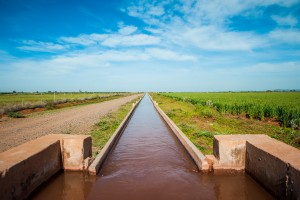
\includegraphics[width=12cm]{amenagementHydraulique.jpg} \\
        \footnotesize
        Source : \href{https://ormvah.com/amenagement-service-eau/amenagement-en-petite-et-moyenne-hydraulique/}{https://ormvah.com/}

        \vfill
    \end{center}

    %Paramètre
    \begin{tabular}{ll}
        Auteur :  & \etudiant \\
        Date :    & \annee \\
        Version : & \textbf{PROVISOIRE}
    \end{tabular}
\end{titlepage}
    \restoregeometry

    %\vfill
\begin{center}
    \Huge Préambule
\end{center}
\vspace{1cm}
Ce travail de Bachelor (ci-après dénommé TB) est réalisé à la fin du cursus d'études, en vue de l'obtention du titre de Bachelor of Science HES-SO en Ingénieurie.
\newline \newline
En tant que travail académique, son contenu, sans préjuger de sa valeur, n'engage ni la responsabilité de l'auteur, ni celles du jury du travail de Bachelor et de la HEIG-VD et HES-SO.
\newline \newline
Toute utilisation, même partielle, de ce TB doit être faîte dans le respect du droit d'auteur.
\vspace{1cm}
HEIG-VD
Le Doyen du département EC+G
\vfill

    % Première partie (numérotation en chiffres romain)
    \pagestyle{front}  
    \tableofcontents
    \newpage

    % Deuxième partie (numérotation en chiffres arabes)
    \thispagestyle{main}

    \chapter{Introduction}

\section{Divers types de débits}
\begin{figure}[H]
    \centering
    \subfigure[\label{fig:debitEtiage} Etiage \textit{ou basse eau} (\LS{15})]{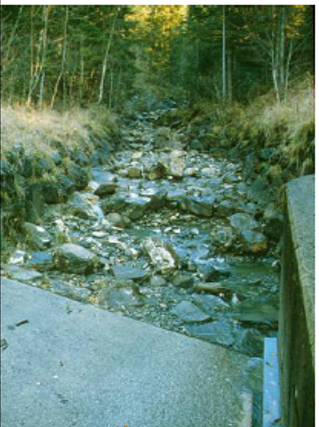
\includegraphics[height=7cm]{etiage.png}}
    \subfigure[\label{fig:debitNormal} Débit normal \textit{ou morphogène} (\MH{0.7})]{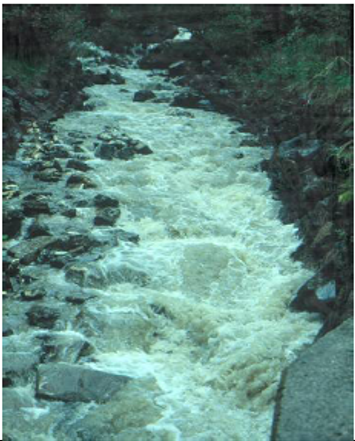
\includegraphics[height=7cm]{debitNormal.png}}
    \subfigure[\label{fig:debitCrue} Crues (\MH{10})]{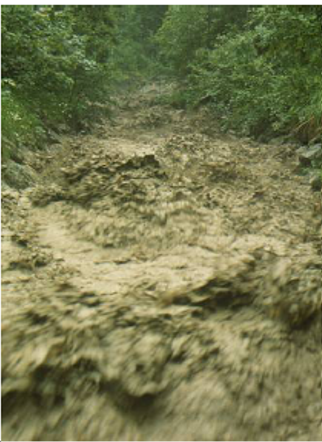
\includegraphics[height=7cm]{crue.png}}
    \caption{Différentes dénominations de débits}
    \label{fig:debits}
\end{figure}

\begin{itemize}
    \item \underline{\textbf{Débit d'étiage :}} quand les rivières tombent à sec ou presque.
    Il est important de connaître ces valeurs minimales dans un cours pour gérer toutes les demandes en matière de prélèvement d'eau, d'écoulement permanent à restituer en aval d'un barrage.
    La législation suisse parle d'un débit $Q_{347}$ (débit moyen sur une journée dépassé en moyenne 347 jours dans une année).
    \item \underline{\textbf{Débit morphogène :}} les érosions des berges sont normalement influencées par ces mêmes débits. Cela dépend aussi des caractéristiques locales comme la granulométrie du fond du lit.
    \item \underline{\textbf{Crue :}} important de connaître le débit pour pouvoir définir les zones de risques au sens de la législation suisse (cf. unité de cours \texttt{Hydraulique 2}).
\end{itemize}

\section{Débits et temps de retour}
\begin{itemize}
    \item Une crue qui survient en moyenne 1 fois tous les 100 ans affiche donc un temps de retour centennal.
    On peut aussi parler de $Q_{100}$.
    \item La probabilité moyenne associée à ce temps de retour d'être atteinte ou dépassée est de 1/100.
    \item Les lois et recommandations fédérales obligent des protections en fonction des temps de retours (cf. Figure \ref{fig:matriceProtection}).
\end{itemize}
\begin{figure}[h!]
    \centering
    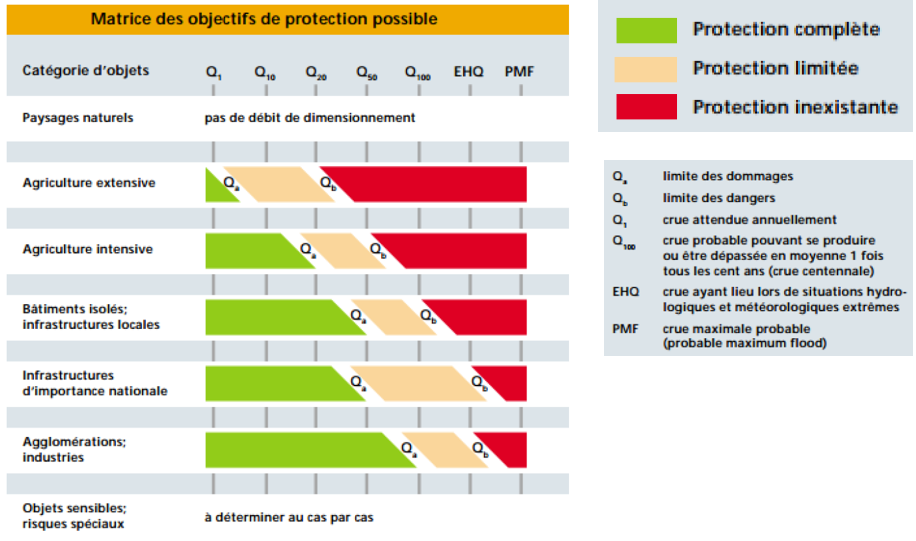
\includegraphics[width=10cm]{matriceObjectifsDimensionnement.png}
    \caption{Matrice de protection possible}
    \label{fig:matriceProtection}
\end{figure}

\section{Méthodes d'analyse et de calculs}
\begin{enumerate}
    \item Analyse statistique avec veille hydrologique
    \item Modèle conceptuel avec des corrélations exprimant les débits de dimensionnement en fonction des paramètres physiques et morphologiques du bassin versant
\end{enumerate}
    \chapter{Analyse de séries de données de débits}

\section{Explication}

\section{Séries annuelles, avec débits maximaux}
\fbox{ %fbox est utilisé pour voir les bords de la minipage
    \begin{minipage}[l]{17cm}
        L'étude est la marche à suivre conviennet pour des séries statistiques avec un débit maximal annuel ! \\
        Cela veut dire que pour chaque année (et chaque mois) nous avons le débit maximal, le tout sur une période donnée (plusieurs années) (ex. Tab. \ref{tab:serieAnnuelleMaximum})
    \end{minipage}
}

\begin{table}[H]
    \centering
    \begin{tabular}{|c||c|c|c|c|c|c|c|c|c|c|c|c|}
        \hline
        \textbf{Année} & \textbf{Jan} & \textbf{Fev} & \textbf{Mar} & \textbf{Avr} & \textbf{Mai} & \textbf{Juin} & \textbf{Jui} & \textbf{Aoû} & \textbf{Sep} & \textbf{Oct} & \textbf{Nov} & \textbf{Dec} \\
        \hline \hline
        \textbf{1965}  & 11 & 10 & 14 & 15 & 160 & 205 & 205 & \cellcolor{red}350 & 145 &  84 &  21 & 18 \\
        \hline
        \textbf{1966}  & 17 & 19 & 17 & 47 & 105 & \cellcolor{red}175 & 155 & 150 &  97 & 125 &  25 & 20 \\
        \hline
        \textbf{1967}  & 17 & 19 & 20 & 39 & 145 & \cellcolor{red}320 & 240 & 210 & 110 &  75 &  38 & 35 \\
        \hline
        \textbf{1968}  & 19 & 15 & 21 & 53 & 125 & 205 & \cellcolor{red}220 & 115 & 140 &  57 & 185 & 40 \\
        \hline
        \textbf{1969}  & 15 & 13 & 14 & 32 & 120 & \cellcolor{red}205 & 190 & 175 &  82 &  65 &  45 & 22 \\
        \hline
        \textbf{\dots} &    &    &    &    &     &     &     &     &       &     &     &      \\
        \hline
        \textbf{1992}  & 14 & 13 & 17 & 62 & 110 & \cellcolor{red}290 & 225 & 215 & 175 &  75 &  46 & 38 \\
        \hline
        \textbf{1993}  & 28 & 42 & 38 & 49 & 125 & 200 & 180 & 150 & \cellcolor{red}460 & 170 &  37 & 27 \\
        \hline
    \end{tabular}
    \caption{Tableau avec les débits maximums pour chaque mois entre les années 1965 et 1993}
    \label{tab:serieAnnuelleMaximum}
\end{table}

\subsection{Procédure pour déterminer et extrapoler les temps de retour}
\begin{enumerate}
    \item \textbf{\underline{Vérification de la stationnarité des données statistiques :}} \\
    \begin{itemize}
        \item Graphique des débits maximum par années
        \item Vérification que cela ne varie par en fonction des années (courbe de tendance)
        \item Visualiser l'évolution des crues de pointe en fonction des années donne un bon aperçu d'une dérive quelconque
        \item \Warning Si les données ne sont pas stationnaires ; cela ne sert à rien de continuer la procédure pour déterminer les débits extrapolés
    \end{itemize}
    \bigskip
    \item \textbf{\underline{Vérification de l'homogénéité des données statistiques :}}
    \begin{itemize}
        \item Vérification optionnelle (car implique d'avoir les débits maximaux mensuels)
        \item Vérification que cela ne varie par en fonction des années (courbe de tendance)
        \item Visualiser l'évolution des crues de pointe en fonction des années donne un bon aperçu d'une dérive quelconque
    \end{itemize}
    \bigskip
    \item \textbf{\underline{Calcul des temps de retour $T$ :}}
    \begin{enumerate}
        \item Classer les débits par ordre décroissant (du plus grand au plus petit)
        \item Inscrire le rang de chaque débit
        \item Calculer le temps de retour selon la formule choisie (cf. Tab. \ref{tab:formuleTempsRetour}) \\
        Conseil : utiliser la formule de Hazen
    \end{enumerate}
    \item \textbf{\underline{Calcul des paramètres de la loi de Gumbel :}} \\
    \textit{Appelé aussi ajustement statistiques} 
    \begin{enumerate}
        \item Calcul de la fonction $F(Q_{obs})$
        \item Calcul des divers paramètres des données statistiques :
        \begin{itemize}
            \item Moyenne des débits observés {\color{red} $\bar{Q}_{obs} = \Sigma Q_{obs_{i}}$}
            \item Ecart-type de la moyenne {\color{red} $\sigma_{Q_{obs}}$ (\texttt{Excel : "ECARTYPE.STANDARD()"})}
            \item Paramètre $a = \bar{Q}_{obs} - 0.5772 \cdot b$
            \item Paramètre $b = \cfrac{\sqrt{6}}{\pi} \cdot \sigma_{Q_{obs}}$
        \end{itemize}
        \item Calcul du débit $Q_{Gumbel} = a + b\cdot U$ \\
        Avec $U = -\ln \left( -\ln \left( F(Q_{obs}) \right) \right)$
        \item Créer le graphique :
    \end{enumerate}
    \item \textbf{\underline{Extrapolation d'un débit en fonction du temps de retour :}}
    \begin{enumerate}
        \item Reprendre les paramètres $a$ et $b$ déterminer plus tôt
        \item Fixer les temps de retour $T_{extrapolé}$ souhaités (5, 10, 20, 30, 50, 100, 300 ans)
        \item Calcul de $F(Q) = 1-\cfrac{1}{T_{extrapolé}}$
        \item Calcul de $U = -\ln \left( -\ln \left( F(Q) \right) \right)$
        \item Calcul de $Q_{extrapolé} = a + b \cdot U$
    \end{enumerate}
\end{enumerate}

\begin{table}[h!]
    \centering
    \begin{tabular}{ccc}
        \toprule
        \textbf{Nom} & \textbf{Formule}            & \textbf{Notes}     \\
        \toprule
        Weibull      & $\cfrac{n+1}{r}$            & Utilisée aux USA   \\
        \midrule
        Médiane      & $\cfrac{n+0.365}{r-0.3175}$ &                    \\
        \midrule
        Hosking      & $\cfrac{n}{r-0.35}$         &                    \\
        \midrule
        Blom         & $\cfrac{n+0.25}{r-0.375}$   &                    \\
        \midrule
        Cunnane      & $\cfrac{n+0.20}{r-0.40}$    &                    \\
        \midrule
        Gringorten   & $\cfrac{n+0.12}{r-0.44}$    &                    \\
        \midrule
        Hazen        & $\cfrac{n}{r-0.5}$          & Utilisée en France \\
        \bottomrule
    \end{tabular}
    \caption{Récapitulatif des formules pour calculer les temps de retour}
    \label{tab:formuleTempsRetour}
\end{table}


\section{Séries gonflées}
\section{Séries tronquées}
        

    % Troisième partie (chapitres plus numérotés)
    \pagestyle{back}
    \appendix
    \chapter{Formules}

\section{Temps de retour}
\begin{table}[H]
    \centering
    \begin{tabular}{ccc}
        \toprule
        \textbf{Nom} & \textbf{Formule}            & \textbf{Notes}     \\
        \toprule
        Weibull      & $\cfrac{n+1}{r}$            & Utilisée aux USA   \\
        \midrule
        Médiane      & $\cfrac{n+0.365}{r-0.3175}$ &                    \\
        \midrule
        Hosking      & $\cfrac{n}{r-0.35}$         &                    \\
        \midrule
        Blom         & $\cfrac{n+0.25}{r-0.375}$   &                    \\
        \midrule
        Cunnane      & $\cfrac{n+0.20}{r-0.40}$    &                    \\
        \midrule
        Gringorten   & $\cfrac{n+0.12}{r-0.44}$    &                    \\
        \arrayrulecolor{red} \midrule
        Hazen        & $\cfrac{n}{r-0.5}$          & Utilisée en France \\
        \bottomrule
    \end{tabular}
    \caption{Différentes formules de calculs des temps de retour. $n$ est le nombre d'années total de l'étude; $r$ est le rang}
    \label{tab:formuleTempsRetour}
\end{table}

\section{Loi de Gumbel -- Séries annuelles}
\begin{table}[H]
    \centering
    \begin{tabular}{c|c|c|c}
        \# & \textbf{Paramètres}                & \textbf{Formules}                                                                                                                         & \textbf{Commentaires}      \\
        \hline
        1  & $\overline{Q}_\text{mes}$          & $\overline{Q}_\text{mes} = \cfrac{1}{n} \cdot \displaystyle{\sum_{i=0}^{n} Q_i}$                                                          & Moyenne des débits mesurés \\
        \hline
        2  & $\sigma_{\overline{Q}_\text{mes}}$ & $\sigma_{\overline{Q}_\text{mes}} = \sqrt{\cfrac{1}{n} \cdot \displaystyle{\sum_{i=0}^{n} \left(Q_i - \overline{Q}_\text{mes}\right)^2}}$ & Ecart-type de la moyenne des débits mesurés \\
        \hline
        3  & $a$                                & $a = \overline{Q}_\text{mes} - 0.5772 \cdot b$                                                                                            & \\
        \hline
        4  & $b$                                & $b = \cfrac{\sqrt{6}}{\pi} \cdot \sigma_{\overline{Q}_\text{mes}}$                                                                        & \\
        \hline
        5  & $F(Q)$                             & $F(Q) = 1-\cfrac{1}{T}$                                                                                                                   & \\
        \hdashline                   
        6  & $F(Q)$                             & $F(Q) = e^{-e^{\frac{- \left(Q-a\right)}{b}}}$                                                                                            & \\
        \hline
        7  & $Q$                                & $Q = a + b \cdot U$                                                                                                                       & Débit selon la loi de Gumbel \\
        \hline
        8  & $U$                                & $U = -\ln \left[ -\ln \left(F(Q)\right)\right]$                                                                                          & Variable réduite de Gumbel   \\
    \end{tabular}
    \caption{Ajustement statistique par la loi de Gumbel}
    \label{tab:loiGumbel}
\end{table}

\section{Loi de Gumbel -- Séries tronquées}
\begin{table}[H]
    \centering
    \begin{tabular}{c|c|c|c}
        \# & \textbf{Paramètres}                & \textbf{Formules}                                                                                                                         & \textbf{Commentaires}      \\
        \hline
        1  & $\overline{Q}_\text{mes}$          & $\overline{Q}_\text{mes} = \cfrac{1}{n} \cdot \displaystyle{\sum_{i=0}^{n} Q_i}$                                                          & Moyenne des débits mesurés \\
        \hline
        2  & $\sigma_{\overline{Q}_\text{mes}}$ & $\sigma_{\overline{Q}_\text{mes}} = \sqrt{\cfrac{1}{n} \cdot \displaystyle{\sum_{i=0}^{n} \left(Q_i - \overline{Q}_\text{mes}\right)^2}}$ & Ecart-type de la moyenne des débits mesurés \\
        \hline
        3  & $a_\text{exp}$                     & $a_\text{exp} = \overline{Q}_\text{mes} - b_\text{exp}$                                                                                   & \\
        \hline
        4  & $b_\text{exp}$                     & $b_\text{exp} = \sigma_{\overline{Q}_\text{mes}}$                                                                                         & \\
        \hline
        5  & $\lambda$                          & $\lambda = \cfrac{\text{nombre de débits}}{\text{nombre de valeurs}}$                                                                     & \\                                               
        \hline
        6  & $a$                                & $a = a_\text{exp} + b_\text{exp} \cdot \ln \left(\lambda\right)$                                                                          & \\                                                                                         
        \hline
        7  & $b$                                & $b = b_\text{exp}$                                                                                                                        & \\
        \hline
        8  & $F(Q)$                             & $F(Q) = 1-\cfrac{1}{T}$                                                                                                                   & $T = \cfrac{1}{1-F(Q)} \\
        \hdashline                   
        9  & $F(Q)$                             & $F(Q) = e^{-e^{\frac{- \left(Q-a\right)}{b}}}$                                                                                            & \\
        \hline
        10  & $Q$                               & $Q = a + b \cdot U$                                                                                                                       & Débit selon la loi de Gumbel \\
        \hline
        11 & $U$                                & $U = -\ln \left[ -\ln \left(F(Q)\right)\right]$                                                                                          & Variable réduite de Gumbel   \\
    \end{tabular}
    \caption{Ajustement statistique par la loi exponentielle et la loi de Gumbel}
    \label{tab:loiGumbelAjuste}
\end{table}

\section{Conversion volumes et débits}
\begin{table}[h!]
    \centering
    \begin{tabular}{|c|c|c|c|c|c|c|c|c|c|c|c|}
        \hline
        \multicolumn{3}{|c|}{\textbf{$m^3$}} & \multicolumn{3}{|c|}{\textbf{$dm^3$}} & \multicolumn{3}{|c|}{\textbf{$cm^3$}} & \multicolumn{3}{|c|}{\textbf{$mm^3$}} \\
        \hline
         & &                                 & $hL$ & $daL$ & $L$                    & $dL$ & $cL$ & $mL$                    & & & \\
        \hline \hline
         & &                               1 & 0    &   0   & 0                      & & &                                   & & & \\  
        \hline
         & &                              0. & 0    &   0   & 1                     & & &                                   & & & \\
        \hline
    \end{tabular}
\end{table}

\begin{align*}
    \MS{1} &= \LS{1000}   \\
           &= \MH{3.6e3} \\
           &= \LH{3.6e6} \\
\end{align*}

    \chapter{Calculer un $Q$ pour un $T_\text{retour}$ donné -- \textit{Séries annuelles}}


    
    %\listoffigures
    %\listoftables

    %\printindex

\end{document}


% Structure normale :
% -> Page de garde
% -> Dédicaces et remerciements
% -> Table des matières
% -> Liste des figures et des tableaux
% -> Préface
% -> Corps du texte
% -> Bibliographie
% -> Annexes
% -> Glossaire et index